\begin{figure}
\centering
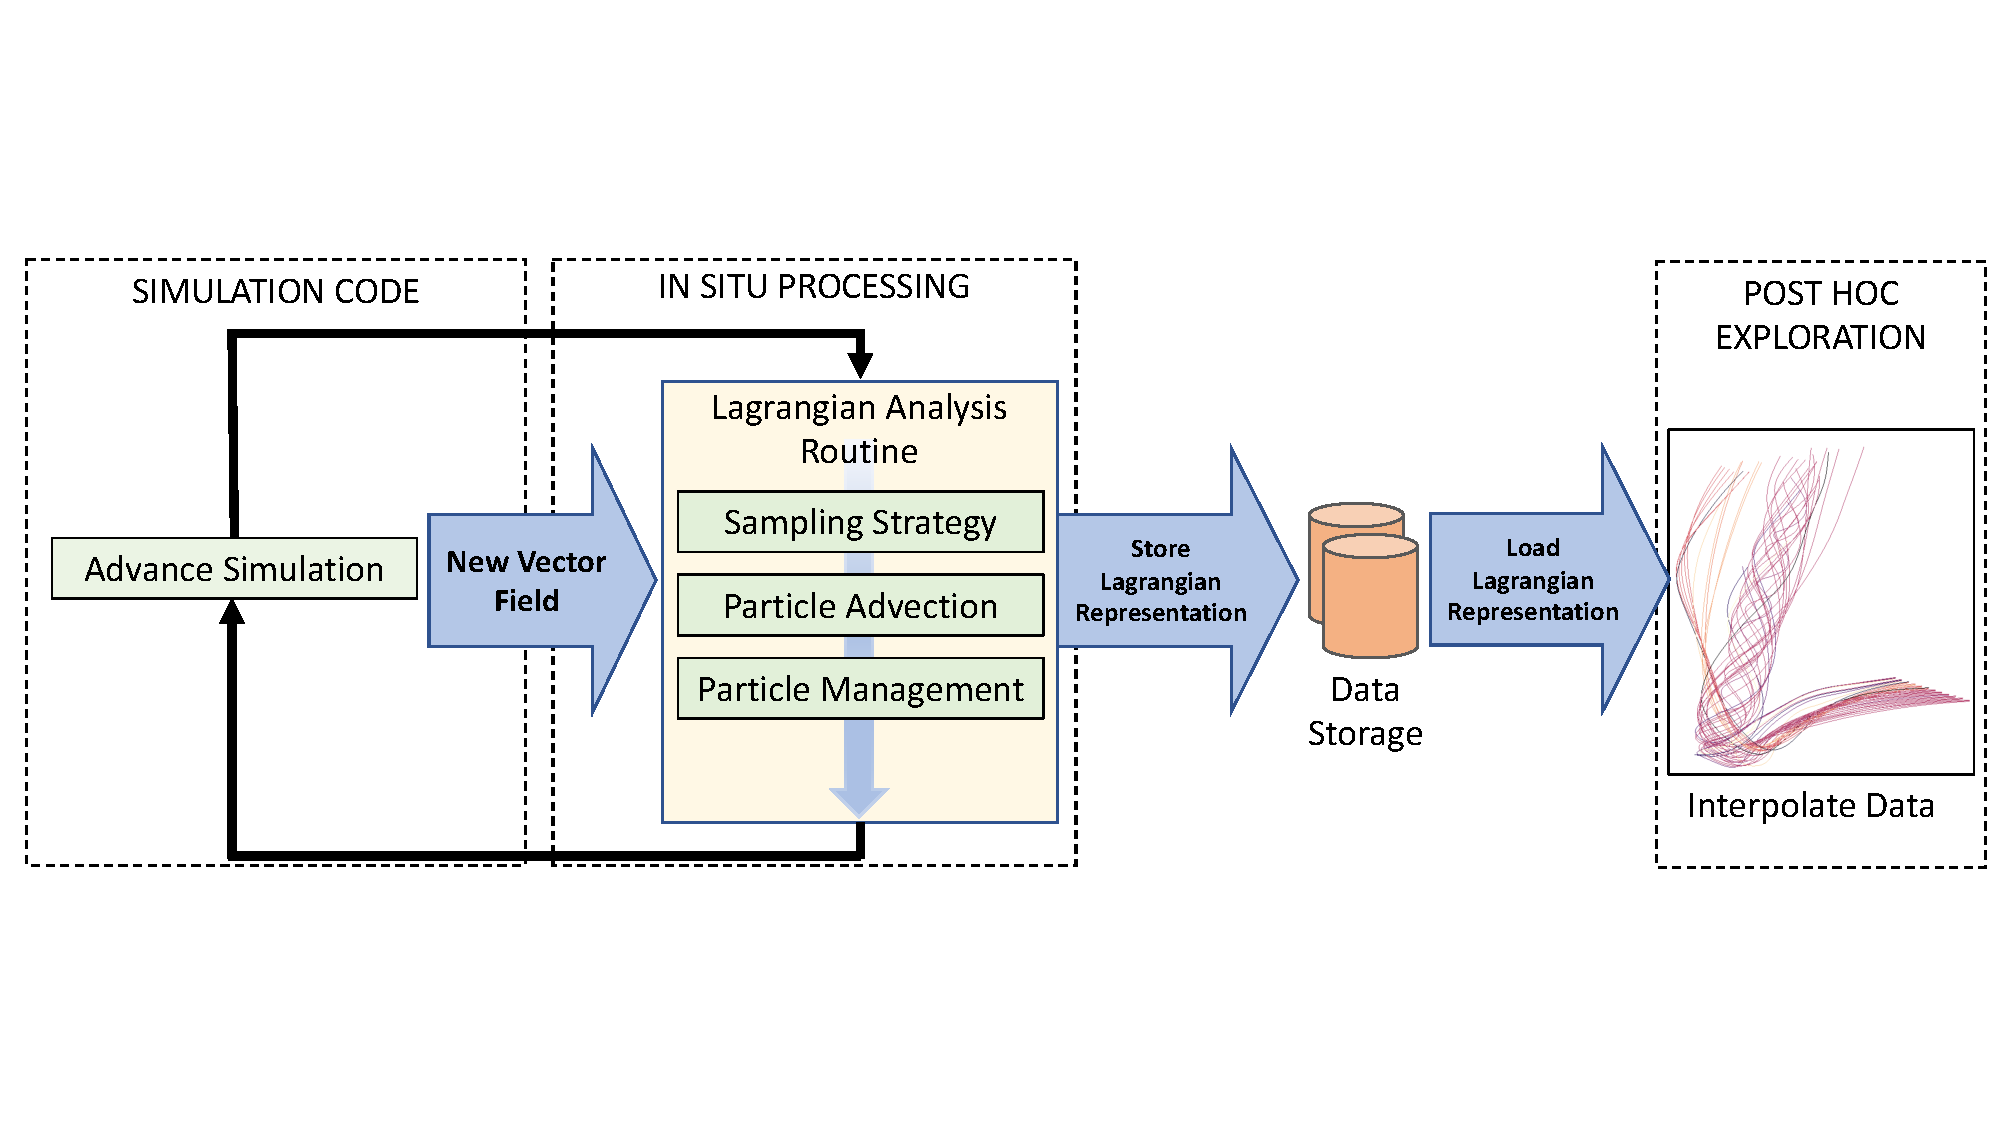
\includegraphics[width=\linewidth,trim={0cm 4.3cm 0cm 4.3cm}, clip ]{images/Schematic.pdf}
\vspace{-6mm}
\caption{Schematic diagram of the \textbf{L-ISR-PHE} workflow showing \textit{in situ} processing, data storage, and \textit{post hoc} exploration.}
\label{fig:schematic}
\vspace{-6mm}
\end{figure}

This section describes considerations for an empirical study of the \textbf{L-ISR-PHE} workflow.
%
Specifically: 
\begin{tightItemize}
\item Subsection~\ref{sec:instantiation} describes the instantiation we consider. 
\item Subsection~\ref{sec:eval} describes evaluation criteria.
\item Subsection~\ref{sec:workloads} describes important factors in defining workloads.
\end{tightItemize}

%This section describes our specific choice of instantiation for each of the components of the \textbf{L-ISR-PHE} workflow, i.e., in \textit{situ reduction}, data storage, and \textit{post hoc} exploration. 
%%
%
%Our discussion includes, when applicable, identifying ``areas'' to evaluate the components.
%
%We encode these in parentheses and name them based on the component they relate to.
%
%Next, in Section~\ref{sec:parameters} we discuss the parameter space we explore and identify which ``areas'' of the \textbf{L-ISR-PHE} workflow it impacts. 




%In this section, we first identify the evaluation areas for the in situ reduction, data storage, and post hoc exploration components of the \textbf{L-ISR-PHE} workflow.
%%
%%
%Next, in Section~\ref{sec:instantiation} we specify our choice of instantiation for each of the components.
%
%\subsection{\textbf{L-ISR-PHE Workflow}}
%The \textbf{L-ISR-PHE} workflow has multiple components (schematic in Figure~\ref{fig:schematic}) that we discuss in the following subsections. 
%

\subsection{Instantiation}
\label{sec:instantiation}

Figure~\ref{fig:schematic} shows a high-level description of the
\textbf{L-ISR-PHE}  workflow.
%
There are many possible strategies for accomplishing the components
within this workflow, i.e., sampling strategy, particle management,
storage, and interpolation.
%
That said, we focus this empirical study on 
the current best practices in this space.
%

%This phase involves 
%At a high-level, extracting a Lagrangian representation involves a domain sampling strategy, performing advection every cycle of the simulation, and other particle management tasks (validating, storing, etc.).
%%
%Our empirical study adopts currently known best practice techniques to extract a Lagrangian representation at scale.
%
%For a domain sampling strategy, we adopt the

\textbf{\textit{In Situ} Reduction:}
\textit{In situ} reduction operates by maintaining a set of particles and their
trajectories.
%
As the simulation completes each cycle, it then invokes our visualization 
routines to update particle positions to reflect the advancement in time.
%
The main decisions for our visualization routines
 are when and where to introduce particles,
when to terminate particles, and what information to save about particles.
%
For this empirical study, we introduced particles using the 
uniform seed placement scheme from Agranovksy et al.~\cite{agranovsky2014improved}, including re-introducing particles at fixed intervals.
%
Our particle termination follows the 
communication-free model from Sane et al.~\cite{sane2020scalable}, where
particles are terminated either if they reach the end of the interval
of if they exit the block.
%
While this captures less information at the block boundaries, results show
that the overall loss of accuracy is very low, 
and the \textit{in situ} encumbrance is much reduced.
%
%The specific details of our implementation are in Section~\ref{sec:insituimp}.
%For each particle, we store only its final position, as its seed location
%can be represented implicitly.

\textbf{Data Storage:}
%
Lowering the encumbrance on file data storage systems is one of the primary motivators to use the \textbf{L-ISR-PHE} workflow.
%
Data storage costs can vary based on 1) how many particles are used to sample the domain, and 2) what information is stored for each particle.
%
Typically, when using more particles, and thus more data storage, a stakeholder would expect greater integrity during exploration.
%
Further, the efficacy of exploration can be closely tied to the nature of the stored data.
%
Although the general \textbf{L-ISR-PHE} framework can support complex Lagrangian reprensentations (unstructured particle sets, polynomial expressions, attribute information, etc.), these are yet unexplored. 
%
For our empirical study, a particle trajectory in the Lagrangian representation is stored using a start and end location of the trajectory during the interval of calculation, similar to previous works~\cite{agranovsky2014improved, sane2018revisiting, sane2020scalable}.
%
These saved particle trajectories are called ``basis flows.''
%

\textbf{\textit{Post Hoc} Exploration:}
The final phase of the \textbf{L-ISR-PHE} workflow involves 
exploratory flow visualization, which in turn requires
constructing new particle trajectories.
%
These new particles trajectories are constructed by 
interpolating from the basis flows.
%interpolating the information extracted to generate new time-dependent vector field visualizations.
%
As mentioned in the discussion of storage, 
the efficacy of the technique is dependent on the nature of the data stored.
%
Prior works have looked extensively at the theoretical and empirical error of Lagrangian-based advection schemes~\cite{hlawatsch2011hierarchical, bujack2015lagrangian, hummel2016error, chandler2016analysis, sane2018revisiting} and proposed methods to interpolate long trajectories~\cite{sane2019interpolation} and particles with non-zero mass~\cite{chandler2015interpolation}.
%
The essential operations involved in constructing new particle trajectories 
are identifying which basis flows to interpolate and performing interpolation.
%
Further,  
distributed-memory settings require communication to continue particle trajectory computation across node boundaries. 
%
Depending on whether the Lagrangian representation is structured or unstructured, different search structures are required.
%
We believe evaluating the cost of interpolating an unstructured particle set is more valuable, as it informs the general case.
%
Therefore, for our empirical study, 
we use the Lagrangian-based advection scheme described by Sane et al.~\cite{sane2020scalable}, to perform search structure~(Delaunay triangulation) construction in parallel and operate in a distributed-memory environment.
%
To perform interpolation on unstructured data, multiple scattered point interpolation schemes can be used.
%
However, the choice of interpolation scheme impacts efficacy, and thus, we use Barycentric coordinates, as recommended in a study by Agranovsky et al.~\cite{agranovsky2015subsampling}.


\subsection{Evaluation Criteria}
\label{sec:eval}

We consider evaluation criteria for each component of the workflow:
%\begin{tightItemize}
\textbf{\textit{In situ} reduction:}
\begin{tightItemize}
\item \textbf{ISR-1 Time:} the execution time spent by the simulation on data analysis and visualization. 
\item \textbf{ISR-2 Memory:} the runtime memory used by \textit{in situ} processing. 
\end{tightItemize}
\textbf{Data storage:}
\begin{tightItemize}
\item \textbf{DS-1 Size:} the file storage costs (i.e., bytes). 
\end{tightItemize}
\textbf{\textit{Post hoc} exploration:}
\begin{tightItemize}
\item \textbf{PHE-1 Time:} the execution time spent to construct new particle trajectories from basis flows
(search structure construction, interpolation, communication).
\item \textbf{PHE-2 Accuracy:} the accuracy of interpolated trajectories.
\end{tightItemize}
%\end{tightItemize}

\noindent
We also eliminated some criteria from consideration to limit scope:

\noindent
\textbf{\textit{In situ} reduction:}
We did not add an evaluation criteria to consider the ease of \textit{in situ}
integration.
%
This is an important concern, but we feel that it is beyond the scope
of this study. 
%
Further, there has been significant research on reducing the
burden on simulation codes to incorporate
\textit{in situ} visualization routines\cite{ayachit2016sensei,fogal2014freeprocessing,Larsen2017Ascent,liu2014hello,Vishwanath2011glean},
and so we are confident that this barrier will become
smaller over time.

\noindent
\textbf{Data storage:} We did consider and measure execution time, but found
supercomputing I/O times were very fast for our scale of study and often contained noise, likely due to contention on the supercomputer. 
%highly inconsistent due to contention,
%tension between latency and bandwidth, and other factors.  
More discussion can be found in~\ref{sec:iocost}.
%and other factors, and also performance varies
%based on latency and bandwidth.
%We did measure these as part of our study, and confirm the expected
%results: Lagrangian performance is always better than the traditional
%approach (since less data is being stored), and execution time goes
%down when less data is stored.  However, patterns beyond these broad trends
%are variable.
%We also considered file format challenges, but found that basis flows can be easily
%stored in existing formats.

\noindent
\textbf{\textit{Post hoc} exploration:} We did not consider if and whether Lagrangian-based extracts 
would affect specific flow visualization techniques.
%
For example, are techniques, such as path
surfaces or finite-time Lyapunov exponents, sensitive or insensitive
to the \textbf{L-ISR-PHE} workflow.  
We view this as future work.
%\end{tightItemize}

%
%\subsection{Evaluation Areas}
%\subsubsection{In Situ Reduction}
%\begin{itemize}
%\item \textbf{IS-E3 Ease of integration:} 
%\end{itemize}
%
%\subsubsection{Data Storage}
%\begin{itemize}
%\item \textbf{DS-E1 File size:}
%\item \textbf{DS-E2 File format:}
%\item \textbf{DS-E3 File write/read time:}
%\end{itemize}
%
%\subsubsection{Post Hoc Exploration}
%\begin{itemize}
%\item \textbf{PH-E1 Execution time:}
%\item \textbf{PH-E2 Accuracy:}
%\end{itemize}
%We identify that the in situ reduction phase can be evaluated along the axes of execution time~(\textbf{ISR-1}), memory~(\textbf{ISR-2}), and ease of integration~(\textbf{ISR-3}).
%
%Execution time and memory are critically important to evaluate the in situ encumbrance and we limit our study to these in this empirical study.
%

%Overall, to evaluate the post hoc phase of \textbf{L-ISR-PHE}, we identify the accuracy of interpolation~(\textbf{PHE-1}), and execution time~(\textbf{PHE-2}), i.e., the costs of performing reconstruction (search structure construction, interpolation, communication).

\subsection{Workload Factors}
\label{sec:workloads}
To understand the technique performance characteristics of the \textbf{L-ISR-PHE} workflow, we identified four parameters that when varied produce the workloads we want to evaluate for our empirical study. 
%Our approach to evaluate \textbf{L-ISR-PHE} involves exploring the technical performance characteristics across the parameter space shown in Table~\ref{}.
%Our study considers the following parameters:
\begin{itemize}
\item \textbf{Number of particles:} Our study varies the number of particles initialized per node and thus inform the cost of performing particle advection for varying workloads every cycle of the simulation. Further, the number of particles initialized is directly impacts the size of the data stored to disk and the accuracy of the reconstruction.
%
We specify the number of particles initialized using the notation \textbf{1:X}, where X is the reduction factor.
%
For example, a 1:1 configuration states that one particle is used for every grid point (no reduction) and a 1:8 configuration states that one particle is used for every 8 grid points (12.5\% of the original data size).
%

\textbf{Impacts $\rightarrow$} \textbf{ISR-1}, \textbf{ISR-2}, \textbf{DS-1}, \textbf{PHE-1}, \textbf{PHE-2}

\item \textbf{Interval:} We consider the interval or frequency at which files are stored to disk.
%
For a given total number of simulation cycles, this impacts the total amount of data stored to disk. 
%
Additionally, for the Lagrangian representation, the interval is equal to the integration length of each particle, and can thus, be consequential to the accuracy of reconstruction.
%
%For each configuration, we specify the number of cycles between storing to disk and refer to this as the \textbf{interval}.
%

\textbf{Impacts $\rightarrow$} \textbf{DS-1}, \textbf{PHE-1}, \textbf{PHE-2}

\item \textbf{Grid size:} We consider different grid sizes to measure the \textit{in situ} encumbrance of varying workloads.
%
Different grid sizes will use a different number of particles to sample the domain reasonably accurately.
%
In particular, we are interested in the \textit{in situ} encumbrance when a single compute node is operating on a large number of grid points.
%
An additional benefit of varying grid size is insight into the variation in simulation cycle time and consequently the percentage of time spent on \textit{in situ} processing.

\textbf{Impacts $\rightarrow$} \textbf{ISR-1}, \textbf{ISR-2}, \textbf{DS-1}

\item \textbf{Concurrency:} We consider the costs at various scale (i.e., number of compute nodes, MPI ranks). Further, the simulation codes required different parallelization hardware and thus, across simulation codes we measure the costs of Lagrangian representation extraction using, both, GPUs and CPUs for particle advection.

\textbf{Impacts $\rightarrow$} \textbf{ISR-1}, \textbf{PHE-2}
\end{itemize}
